
\begin{table}
	\centering
	\begin{tabular}{c|c|c|}
		& \textbf{Singular/Total} & \textbf{Per Node}
		\\ \hline
		Value stored & \(N^3\) & \(\frac{N^3}{\#P}\) 
	\end{tabular}
	\caption{Assuming that the grid is threedimensional and has \(N_x=N_y=N_z=N\) grid points in each direction. Contents of the grid structures as a total, and divided on each computational node.}
\end{table}

\tikzstyle{vertex}=[circle,fill=black!25,minimum size=25pt,inner sep=0pt]
\tikzstyle{ghost}=[circle,fill=blue!25,minimum size=25pt,inner sep=0pt]

	
	\begin{figure}
		\centering
		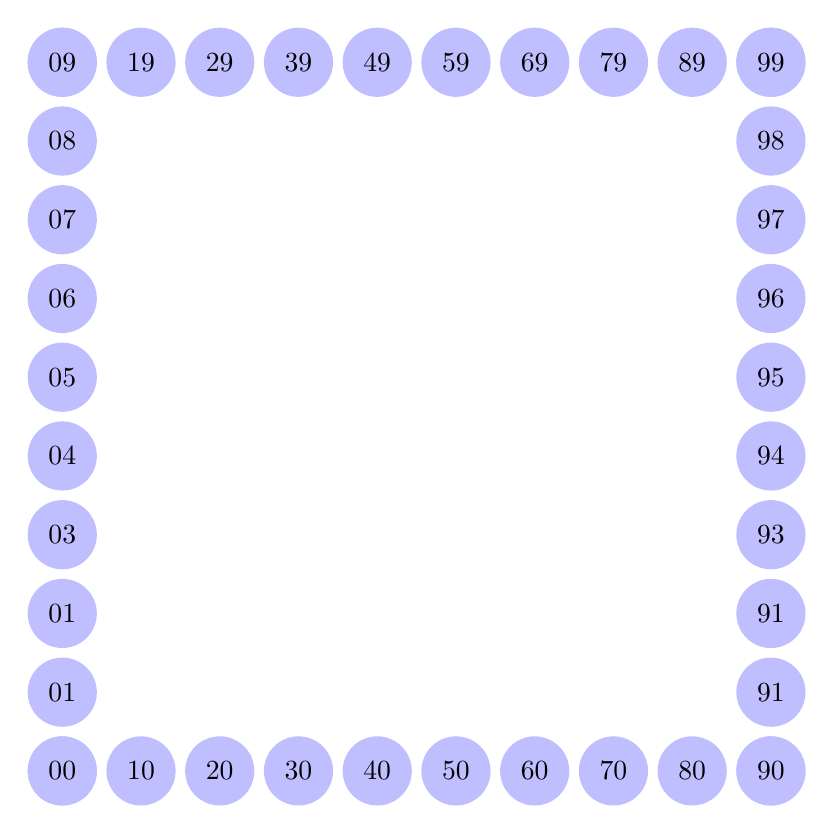
\begin{tikzpicture}[scale=1.0, auto,swap]
			\foreach \pos/\name in 	{}
	    	\node[vertex] (\name) at \pos {$\name$};
	    	%Adding the ghost nodes along the edges
	    	\foreach \pos/\name in 	{{(0,0)/00},	{(1,0)/10}, 	{(2,0)/20},		{(3,0)/30},
	    							 {(4,0)/40},	{(5,0)/50}, 	{(6,0)/60},		{(7,0)/70},
	    							 {(8,0)/80}, 	{(9,0)/90}}
		    \node[ghost] (\name) at \pos {$\name$};
		    \foreach \pos/\name in 	{{(0,0)/00},	{(0,1)/01}, 	{(0,2)/01},		{(0,3)/03},
									{(0,4)/04},		{(0,5)/05}, 	{(0,6)/06},		{(0,7)/07},
									{(0,8)/08}, 	{(0,9)/09}}
		    \node[ghost] (\name) at \pos {$\name$};
		    \foreach \pos/\name in 	{{(0,9)/09},	{(1,9)/19}, 	{(2,9)/29},		{(3,9)/39},
	    							 {(4,9)/49},	{(5,9)/59}, 	{(6,9)/69},		{(7,9)/79},
	    							 {(8,9)/89}, 	{(9,9)/99}}
		    \node[ghost] (\name) at \pos {$\name$};
		    \foreach \pos/\name in 	{{(9,0)/90},	{(9,1)/91}, 	{(9,2)/91},		{(9,3)/93},
									{(9,4)/94},		{(9,5)/95}, 	{(9,6)/96},		{(9,7)/97},
									{(9,8)/98}, 	{(9,9)/99}}
		    \node[ghost] (\name) at \pos {$\name$};
	    \end{tikzpicture}
	    \caption{Hello}
    \end{figure}

	% \begin{figure}
	% 	\begin{subfigure}{1\textwidth}
	% 		\begin{subfigure}[b]{0.18\textwidth}
	% 		\begin{tikzpicture}[scale=1.0, auto,swap]
	%     		\foreach \pos/\name in {{(2,0)/200}, 	{(2,1)/201},	{(2,2)/202},
	%                             		{(1,0)/000}, 	{(1,1)/101}, 	{(1,2)/102},
	%                             		{(0,0)/000}, 	{(0,1)/001},	{(0,2)/002}}
	%         	\node[vertex] (\name) at \pos {$\name$};
	%         \end{tikzpicture}
	%         \caption*{j \(= 0\)}
	%         \end{subfigure}
	%         \qquad \qquad
	%         \begin{subfigure}[b]{0.18\textwidth}
	% 		\begin{tikzpicture}[scale=1.0, auto,swap]
	%     		\foreach \pos/\name in {{(2,0)/210}, 	{(2,1)/211},	{(2,2)/212},
	%                             		{(1,0)/010}, 	{(1,1)/111}, 	{(1,2)/112},
	%                             		{(0,0)/010}, 	{(0,1)/011},	{(0,2)/012}}
	%         	\node[vertex] (\name) at \pos {$\name$};
	%         \end{tikzpicture}
	%         \caption*{j \(= 1\)}
	%         \end{subfigure}
	%         \qquad \qquad
	%         \begin{subfigure}[b]{0.18\textwidth}
	% 		\begin{tikzpicture}[scale=1.0, auto,swap]
	%     		\foreach \pos/\name in {{(2,0)/220}, 	{(2,1)/221},	{(2,2)/222},
	%                             		{(1,0)/020}, 	{(1,1)/121}, 	{(1,2)/122},
	%                             		{(0,0)/020}, 	{(0,1)/021},	{(0,2)/022}}
	%         	\node[vertex] (\name) at \pos {$\name$};
	%         \end{tikzpicture}
	%         \caption*{j \(= 2\)}
	%         \end{subfigure}
	%        	\caption{All the neighbors in a \(3\cross 3\) system divided up into three slices with j constant. The numbers are position in an ijk-grid.}
	%        	\label{fig:neighbor_grid}
	% 	\end{subfigure}
	% 	\begin{subfigure}{1\textwidth}
	% 		\begin{subfigure}[b]{0.18\textwidth}
	% 		\begin{tikzpicture}[scale=1.0, auto,swap]
	%     		\foreach \pos/\name in {{(0,2)/X}, 	{(1,2)/X},	{(2,2)/X},
	%                             		{(0,1)/}, 	{(1,1)/}, 	{(2,1)/},
	%                             		{(0,0)/*}, 	{(1,0)/*},	{(2,0)/*}}
	%         	\node[vertex] (\name) at \pos {$\name$};
	%         \end{tikzpicture}
	%         \caption*{j \(= 0\)}
	%         \end{subfigure}
	%         \qquad \qquad
	%         \begin{subfigure}[b]{0.18\textwidth}
	% 		\begin{tikzpicture}[scale=1.0, auto,swap]
	%     		\foreach \pos/\name in {{(0,2)/X}, 	{(1,2)/X},	{(2,2)/X},
	%                             		{(0,1)/}, 	{(1,1)/O}, 	{(2,1)/},
	%                             		{(0,0)/*}, 	{(1,0)/*},	{(2,0)/*}}
	%         	\node[vertex] (\name) at \pos {$\name$};
	%         \end{tikzpicture}
	%         \caption*{j \(= 1\)}
	%         \end{subfigure}
	%         \qquad \qquad
	%         \begin{subfigure}[b]{0.18\textwidth}
	% 		\begin{tikzpicture}[scale=1.0, auto,swap]
	%     		\foreach \pos/\name in {{(0,2)/X}, 	{(1,2)/X},	{(2,2)/X},
	%                             		{(0,1)/}, 	{(1,1)/}, 	{(2,1)/},
	%                             		{(0,0)/*}, 	{(1,0)/*},	{(2,0)/*}}
	%         	\node[vertex] (\name) at \pos {$\name$};
	%         \end{tikzpicture}
	%         \caption*{j \(= 2\)}
	%         \end{subfigure}
	%        	\caption{Let the center cell interact with the top layer. 'X' represents a cell that the center cell, 'O' has interacted with. '*' represents a cell that will interact with the center cel, 'O' if it undergoes the same scheme as the center cell 'O'.}
	%        	\label{fig:top}
	% 	\end{subfigure}
	% 	\begin{subfigure}{1\textwidth}
	% 		\begin{subfigure}[b]{0.18\textwidth}
	% 		\begin{tikzpicture}[scale=1.0, auto,swap]
	%     		\foreach \pos/\name in {{(0,2)/X}, 	{(1,2)/X},	{(2,2)/X},
	%                             		{(0,1)/*}, 	{(1,1)/}, 	{(2,1)/X},
	%                             		{(0,0)/*}, 	{(1,0)/*},	{(2,0)/*}}
	%         	\node[vertex] (\name) at \pos {$\name$};
	%         \end{tikzpicture}
	%         \caption*{j \(= 0\)}
	%         \end{subfigure}
	%         \qquad \qquad
	%         \begin{subfigure}[b]{0.18\textwidth}
	% 		\begin{tikzpicture}[scale=1.0, auto,swap]
	%     		\foreach \pos/\name in {{(0,2)/X}, 	{(1,2)/X},	{(2,2)/X},
	%                             		{(0,1)/*}, 	{(1,1)/O}, 	{(2,1)/X},
	%                             		{(0,0)/*}, 	{(1,0)/*},	{(2,0)/*}}
	%         	\node[vertex] (\name) at \pos {$\name$};
	%         \end{tikzpicture}
	%         \caption*{j \(= 1\)}
	%         \end{subfigure}
	%         \qquad \qquad
	%         \begin{subfigure}[b]{0.18\textwidth}
	% 		\begin{tikzpicture}[scale=1.0, auto,swap]
	%     		\foreach \pos/\name in {{(0,2)/X}, 	{(1,2)/X},	{(2,2)/X},
	%                             		{(0,1)/*}, 	{(1,1)/}, 	{(2,1)/X},
	%                             		{(0,0)/*}, 	{(1,0)/*},	{(2,0)/*}}
	%         	\node[vertex] (\name) at \pos {$\name$};
	%         \end{tikzpicture}
	%         \caption*{j \(= 2\)}
	%         \end{subfigure}
	%        	\caption{Then we let the center cell interact with the rest of the front, i-direction.}
	%        	\label{fig:front}
	% 	\end{subfigure}
	% 	\begin{subfigure}{1\textwidth}
	% 		\begin{subfigure}[b]{0.18\textwidth}
	% 		\begin{tikzpicture}[scale=1.0, auto,swap]
	%     		\foreach \pos/\name in {{(0,2)/X}, 	{(1,2)/X},	{(2,2)/X},
	%                             		{(0,1)/*}, 	{(1,1)/X}, 	{(2,1)/X},
	%                             		{(0,0)/*}, 	{(1,0)/*},	{(2,0)/*}}
	%         	\node[vertex] (\name) at \pos {$\name$};
	%         \end{tikzpicture}
	%         \caption*{j \(= 0\)}
	%         \end{subfigure}
	%         \qquad \qquad
	%         \begin{subfigure}[b]{0.18\textwidth}
	% 		\begin{tikzpicture}[scale=1.0, auto,swap]
	%     		\foreach \pos/\name in {{(0,2)/X}, 	{(1,2)/X},	{(2,2)/X},
	%                             		{(0,1)/*}, 	{(1,1)/O}, 	{(2,1)/X},
	%                             		{(0,0)/*}, 	{(1,0)/*},	{(2,0)/*}}
	%         	\node[vertex] (\name) at \pos {$\name$};
	%         \end{tikzpicture}
	%         \caption*{j \(= 1\)}
	%         \end{subfigure}
	%         \qquad \qquad
	%         \begin{subfigure}[b]{0.18\textwidth}
	% 		\begin{tikzpicture}[scale=1.0, auto,swap]
	%     		\foreach \pos/\name in {{(0,2)/X}, 	{(1,2)/X},	{(2,2)/X},
	%                             		{(0,1)/*}, 	{(1,1)/*}, 	{(2,1)/X},
	%                             		{(0,0)/*}, 	{(1,0)/*},	{(2,0)/*}}
	%         	\node[vertex] (\name) at \pos {$\name$};
	%         \end{tikzpicture}
	%         \caption*{j \(= 2\)}
	%         \end{subfigure}
	%        	\caption{Then we let the center cell interact with side, j-direction and all the neighboring cells to cell \(111\) is interacted with, or interacts with cell \(111\) when all the cells are run trough.}
	%        	\label{fig:side}
	% 	\end{subfigure}
	% 	\caption{A schematic explanation of the algorithm to go through all the neighboring cells of a neighbor cell.}
	% \end{figure}